% \subsection{Rapid Growth Requires \textit{E. coli} to Increase Both Cell Size and Ribosomal
% Mass Fraction}
% In the right-hand side of \FIG{ribosome_limit}(B) we also find that above about 0.75
% hr$^{-1}$ the growth rate is determined solely by the ribosomal mass fraction
% $\Phi_R$, since $f_a$ is close to 1, and $r_t$ is near its maximal rate
% \citep{dai2016}. While $\Phi_R$ will need to increase in order for cells to
% grow faster, the fractional dependence in \EQ{lam_limited}
% gives little insight into how this scaling is actually achieved by the cell.
%
% It is now well-documented that \textit{E. coli} cells add a constant volume per
% origin of replication, which is robust to a remarkable array of cellular
% perturbations \citep{si2017}. Given the proteomic measurements featured in this
% work, we find that the ribosome copy number also scales in proportion to
% $\langle$\# ori$\rangle$ [\FIG{translation_ecoli_partA}(A)]. However,  an
% increase in ribosome abundance alone is not necessarily sufficient to increase
% growth rate and we also need to consider how $\Phi_R$ varies with $\langle$\#
% ori$\rangle$. As shown in \FIG{translation_ecoli_partA}(B), we find
% that the deviations in protein expression with $\langle$\# ori$\rangle$ are
% largely restricted to regions of ribosomal protein genes. Here we have calculated the position-dependent
% protein expression across the chromosome by a running Gaussian average of
% protein copy number (20 kbp st. dev. averaging window) based on each gene's
% transcriptional start site. These were median-subtracted to account for the
% change in total protein abundance with $\langle$\# ori$\rangle$. This result
% suggests that $\Phi_R$ is also being tuned in proportion to $\langle$\#
% ori$\rangle$ under nutrient-limited growth. Importantly, it is through this
% additional dependence on $\Phi_R$, combined with the exponential increase in
% $\langle$\# ori$\rangle$ that was noted in the previous section, that \textit{E. coli}
% exhibits an exponential increase in cell size with growth rate.

%
% \begin{figure*}
%     \begin{fullwidth}
%     \centering{
%         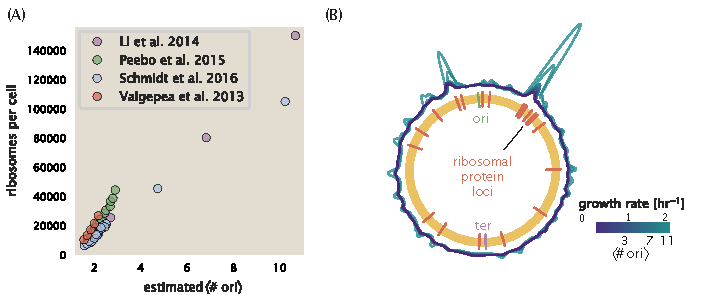
\includegraphics{main_figs/fig11_ribosome_growth_limit_ecoli_a_polar_coord.pdf}
%         \caption{\textbf{Cells increase both absolute ribosome abundance and $\Phi_R$ with
%         $\langle$\# ori$\rangle$.} (A) Plot of the ribosome copy number estimated from the
%         proteomic data against the estimated $\langle$\# ori$\rangle$ (see Appendix
%         Section "Estimation of $\langle$\# ori$\rangle$/ $\langle$\# ter$\rangle$ and $\langle$\# ori$\rangle$ for additional details). (B) A running
%         Gaussian average (20 kbp st. dev.) of protein copy number is calculated
%         for each growth condition considered by \citep{schmidt2016} based
%         on each gene's transcriptional start site. Since total
%         protein abundance increases with growth rate, protein copy numbers are
%         median-subtracted to allow comparison between growth conditions.
%         $\langle$\# ori$\rangle$ are estimated using the data in (A) and
%         Equation \ref{eq:Nori}. } \label{fig:translation_ecoli_partA}
%     }
%     \end{fullwidth}
% \end{figure*}
